\chapter{Results}
In order to discern whether the choice of programming language has an environmental impact, experiments were executed, each time changing a different aspect of the experiment to detect if there was a significant difference between the performance of the languages. Most experiments used the programs to blur 78 high definition images.

\section{C++ and Python with OpenCV }
The first experiment was to run the programs with the chosen profiler of xctrace and cProfile to determine the runtime of each function in the program, blurring 78 images in total. Each benchmark was run five times and then the average was calculated. The average of the results of these experiments is shown in figure 7.1.

\begin{figure}[H]
	\centering
	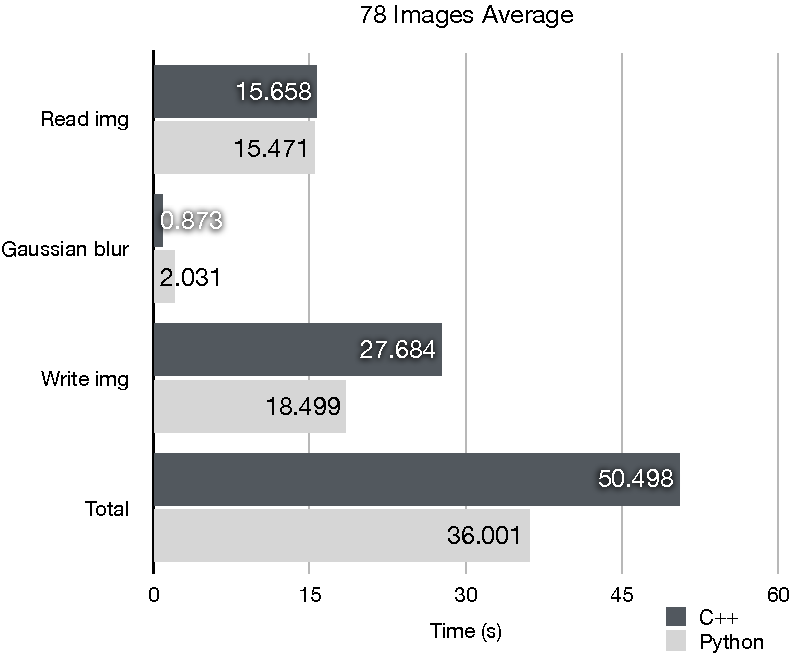
\includegraphics[scale=0.72]{average-without-script.pdf}
	\caption{The average of 5 runs for each language}
	\label{figure:average-78img}
\end{figure}

These results were highly uncharacteristic. Based on previous research, it was expected that C++ would be faster than Python, not slower. Most of the delay for C++ seemed to come from writing the blurred image to the disk, as seen in the write img bars in figure 7.1.

\section{Saving to BMP instead of JPEG}
One approach to solving the significant delay of C++ when writing images to the disk was to change the file type of the image for both languages. The default settings of the OpenCV package saved the image to whichever file type the image had initially been; in this case, that was JPEG (Joint Photographic Experts Group). Changing the file extension from JPEG to BMP (bitmap image file) would change the image file type on saving the image. Strangely, as seen in figure 7.2, this warped the data in such a way that reading the image now took longer for C++ and writing the image was quite a bit faster. It is assumed that this might be attributed to the library version, but further research is needed to confirm this.

\begin{figure}[H]
	\centering
	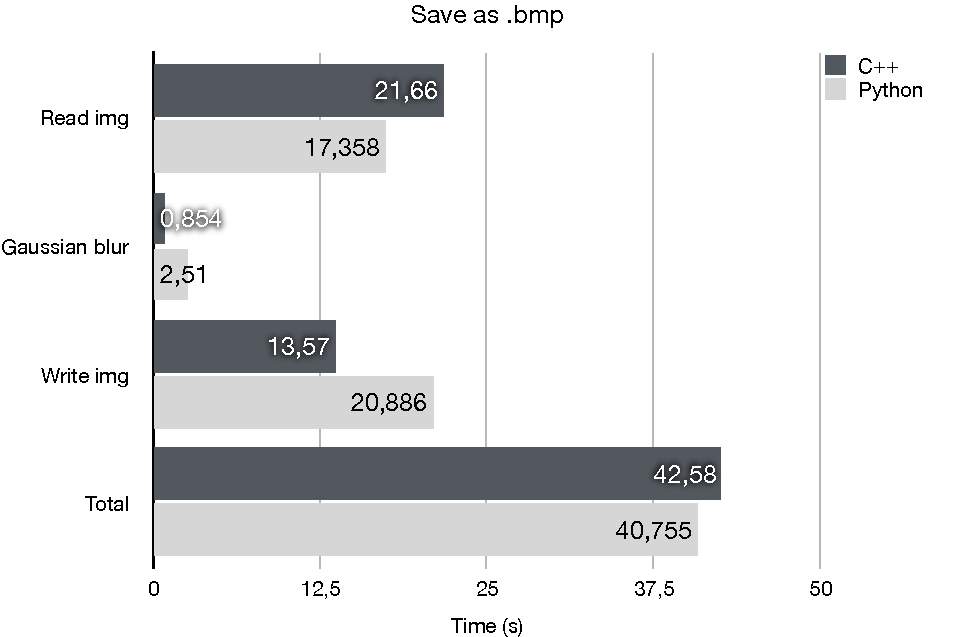
\includegraphics[scale=0.72]{bmp.pdf}
	\caption{Saving the image as a BMP file}
	\label{figure:bmp}
\end{figure}

\section{Using a script to benchmark}
The following experiment was to benchmark the programs using a script. A script is a sequence of instructions that are carried out subsequently by a computer, as seen in listing 5.

\begin{listing}[!ht]
	\begin{minted}[xleftmargin=20pt, linenos]{bash}
#!/bin/bash

#test
python3 ./test_opencv_cprofile.py >> python_profile_test.txt
xctrace record --template 'green' --launch ../C/green_apple_blur_new
/Volumes/RAMDisk/test /Volumes/RAMDisk/test_result
xctrace record --template 'green' --launch ./test_opencv.py

#78 img
python3 ./opencv_cprofile.py >> python_profile.txt
xctrace record --template 'green' --launch ../C/green_apple_blur_new
/Volumes/RAMDisk/raw /Volumes/RAMDisk/cBlurred
xctrace record --template 'green' --launch ./opencv.py
	\end{minted}
	\caption{The script used to profile the different programs}
	\label{listing:script}
	\end{listing}

This was done to minimise the time between running each benchmark and, therefore, minimise the difference between computer operations. It also allowed randomisation of the different programs to see how one program running before or after another might affect its performance.
We can see in figure 7.3-a when compared to figure 7.3-b, that there is a slight difference between the readings when using a script. This is especially visible when writing the image in C++. We might attribute this to the system load caused by running all programs so quickly after each other.

\begin{figure}[H]
	\centering
	\begin{subfigure}{.5\textwidth}
	  \centering
	  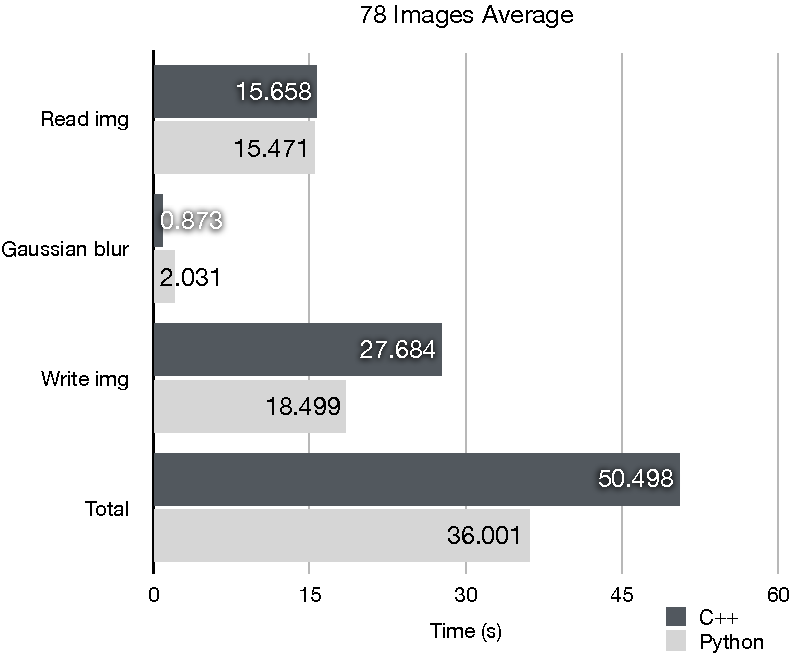
\includegraphics[width=1\linewidth]{average-without-script.pdf}
	  \caption{Average without script}
	  \label{fig:no-script}
	\end{subfigure}%
	\begin{subfigure}{.5\textwidth}
	  \centering
	  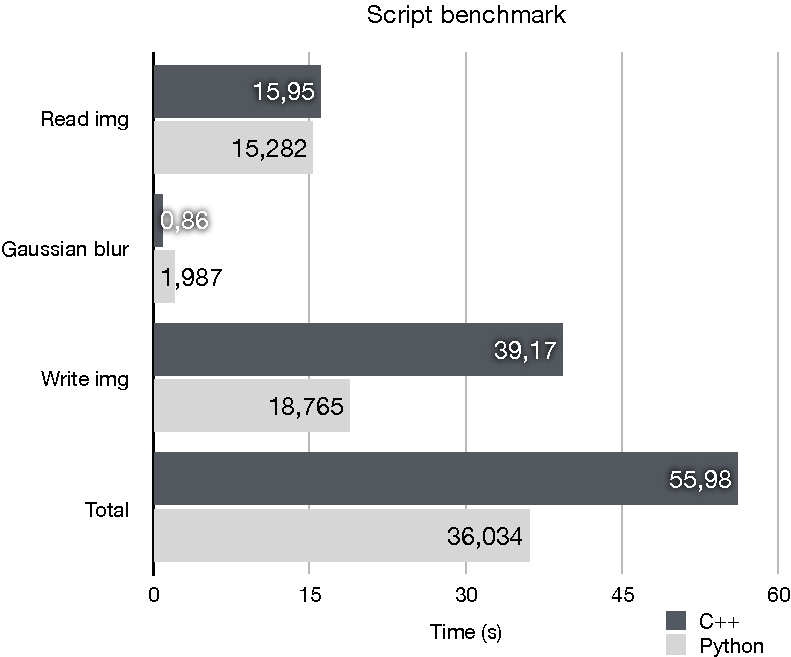
\includegraphics[width=1\linewidth]{script-benchmark.pdf}
	  \caption{Script benchmark}
	  \label{fig:script}
	\end{subfigure}
	\caption{Comparing the results of a script versus no script}
	\label{fig:script-vs-noscript}
\end{figure}

Figure 7.4 shows two benchmarks with a different script order, both using a RAMdisk. Each was measured by blurring 78 images. There is a slight difference between the two benchmarks, the randomised one running about two seconds faster. Overall, the proportions of the different benchmarks stayed the same.

\begin{figure}[H]
	\centering
	\begin{subfigure}{.5\textwidth}
	  \centering
	  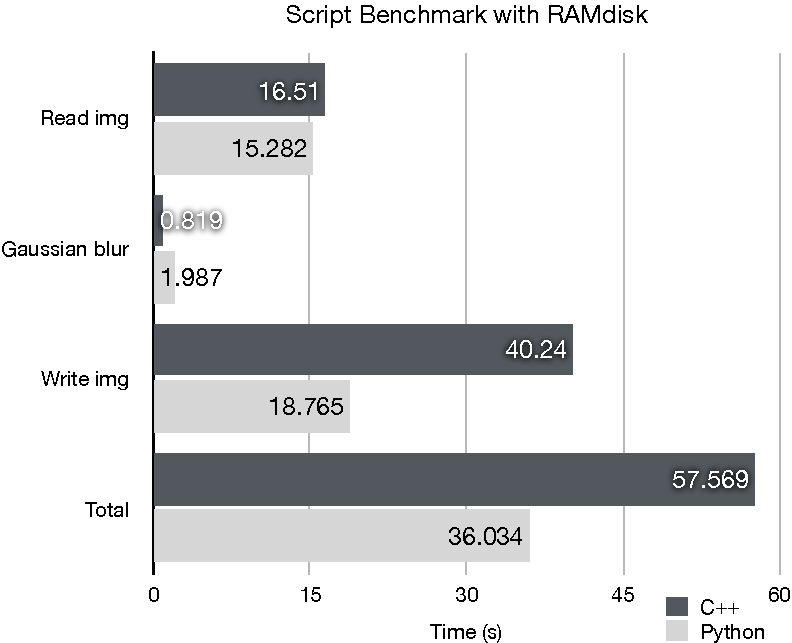
\includegraphics[width=1\linewidth]{ramdisk.pdf}
	  \caption{Script with RAMdisk}
	  \label{fig:ramdisk}
	\end{subfigure}%
	\begin{subfigure}{.5\textwidth}
	  \centering
	  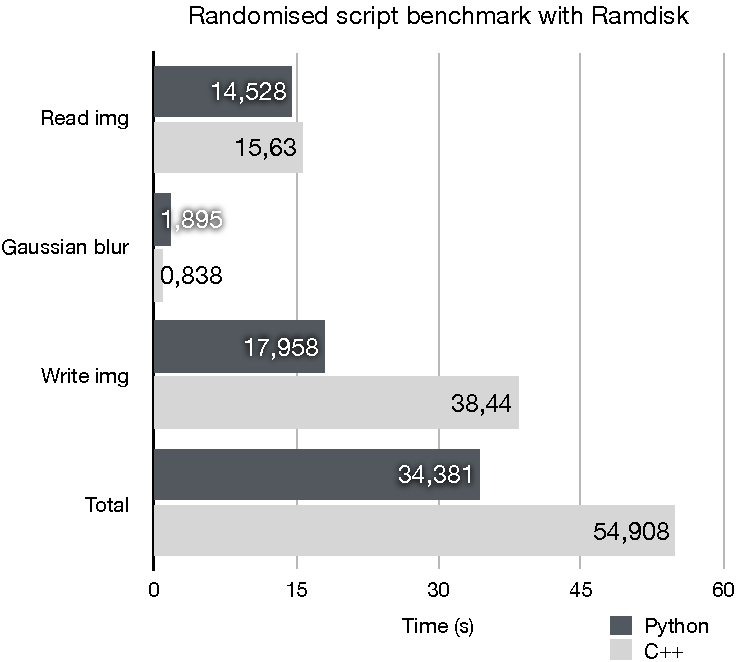
\includegraphics[width=1\linewidth]{random-ramdisk.pdf}
	  \caption{Randomised script with RAMdisk}
	  \label{fig:random-ramdisk}
	\end{subfigure}
	\caption{Comparing two different scripts}
	\label{fig:two-scripts}
\end{figure}

\section{RAMdisk}
A RAMdisk is a block of random-access memory that a computer's software is treating as if the memory were a disk drive. It can be used to accelerate the reading and writing of files. A RAMdisk was installed using the command "diskutil erasevolume HFS+ "RAMDisk" `hdiutil attach -nomount ram://2097152`" in the terminal. This created a RAMdisk with 1 GB of storage space.
As seen in figure 7.5, compared to the benchmarks with no RAMdisk, running the scripted benchmarks with a RAMdisk surprisingly returned a decreased performance. However, the difference is so slight that we cannot confirm whether this is due to the RAMdisk or another influence.

\begin{figure}[H]
	\centering
	\begin{subfigure}{.5\textwidth}
	  \centering
	  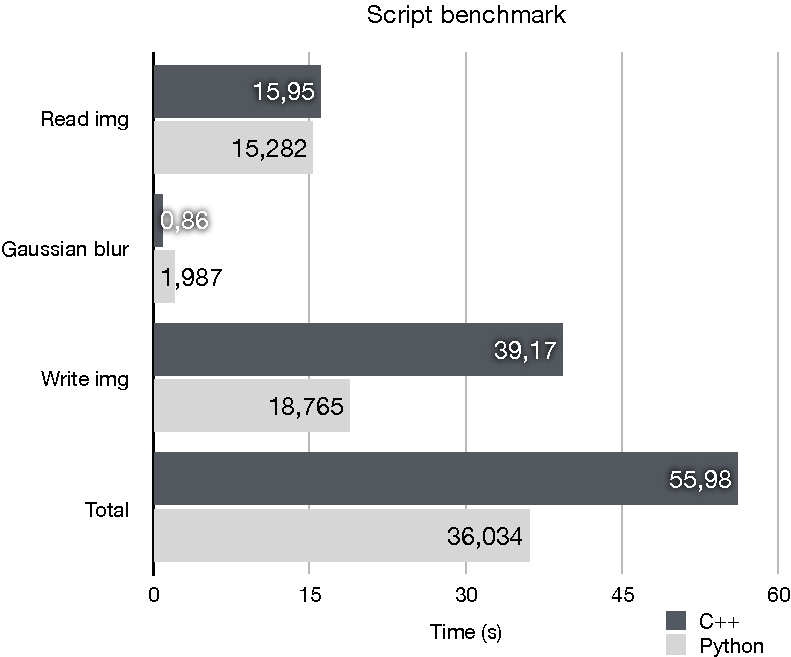
\includegraphics[width=1\linewidth]{script-benchmark.pdf}
	  \caption{Script without RAMdisk}
	  \label{fig:script2}
	\end{subfigure}%
	\begin{subfigure}{.5\textwidth}
	  \centering
	  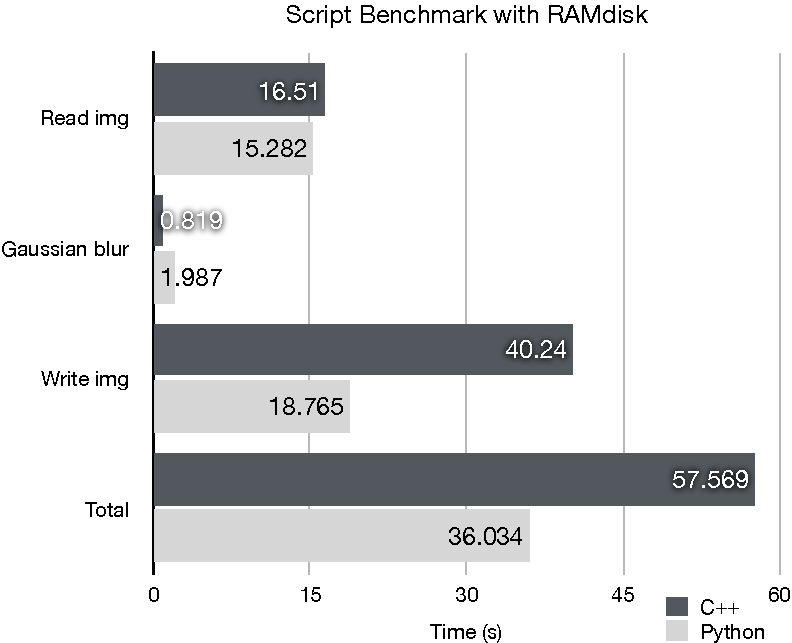
\includegraphics[width=1\linewidth]{ramdisk.pdf}
	  \caption{Script with RAMdisk}
	  \label{fig:ramdisk2}
	\end{subfigure}
	\caption{Comparing benchmarks with and without the use of a RAMdisk using the same script}
	\label{fig:ramdisk-vs-noramdisk}
\end{figure}

\section{Running the programs on a different computer}
In order to detect whether the computer hardware influenced the disk I/O, the programs were tested on a different computer. The same computer type in a different configuration was utilised: the MacBook Pro from 2021 with an M1 Pro Apple Silicon CPU, 32 GB of RAM and a 1 TB SSD (solid-state drive). To run the programs on this new configuration, Python version 3.10.3 needed to be installed instead of the previously used 3.8.12. The software was not compatible with the new M1 chip, so it had to be recompiled for Apple Silicon.
Figure 7.6 shows a similar distribution of runtime for the benchmark but an overall acceleration of 15 to 20 seconds compared to the other computer. These results were expected since this computer was a newer model and had more powerful hardware.

\begin{figure}[H]
	\centering
	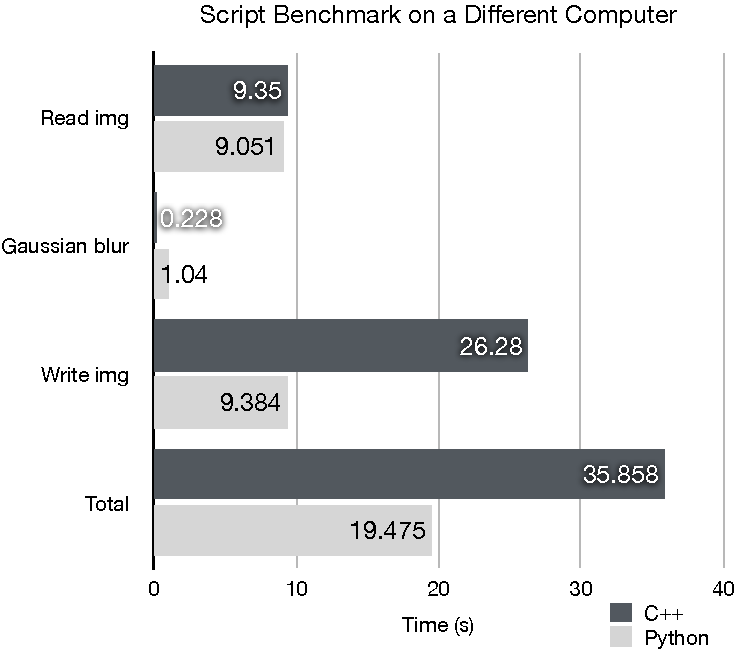
\includegraphics[scale=0.72]{different-comp.pdf}
	\caption{Script benchmark on a different computer}
	\label{figure:different-comp}
\end{figure}

\section{Profiling C++ and Python on Linux}
In order to rule out the possibility of the operating system influencing the unexpectedly slow C++ runtime, it was decided to experiment with the programs on a different operating system. An Ubuntu Linux instance was created using a virtual machine to benchmark the programs. This required some adjusting as the executable made for macOS was not compatible with Linux, and Linux does not support the macOS instruments profiler. The C++ code was compiled with the cmake tool \cite{cmake} to create the new executable. The GCC (GNU Compiler Collection) \cite{gcc} compiler native fprofile command was used as a profiler. For Python, it was still possible to use the cProfile profiler. Each program was run five times and the average was calculated as seen in figure 7.7.
Interestingly, on Linux, the C++ program performed a lot faster than Python, 14.683 seconds faster, to be exact. This might once again be attributed to OpenCV being optimised differently for a different operating system and therefore performing better on Linux.

\begin{figure}[H]
	\centering
	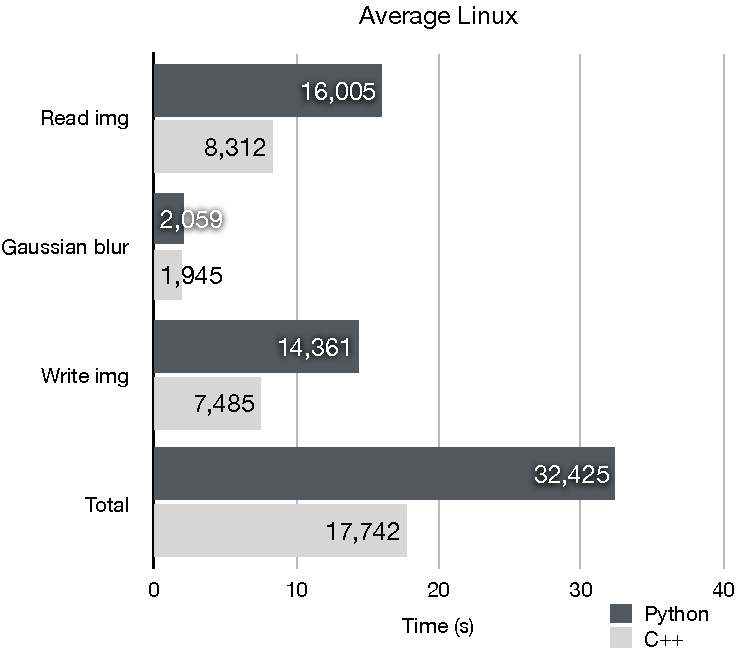
\includegraphics[scale=0.72]{linux.pdf}
	\caption{Average for the programs run on Linux}
	\label{figure:linux}
\end{figure}

\section{C++ using OpenCV from VCPKG}
One theory for the delay of C++ for disk output was that it was due to how the OpenCV library function handled writing to the disk. After doing further research, it was found that the standard OpenCV package for Python is a different version from what is standard for C++. Using VCPKG, a C/C++ dependency manager \cite{vcpkg}, the same version as used for Python was downloaded and used for C++. Benchmarking the programs with 100 randomly generated images shows the results in figure 7.9. Now, we can see only a very insignificant difference between the two programming languages compared to before.

\begin{figure}[H]
	\centering
	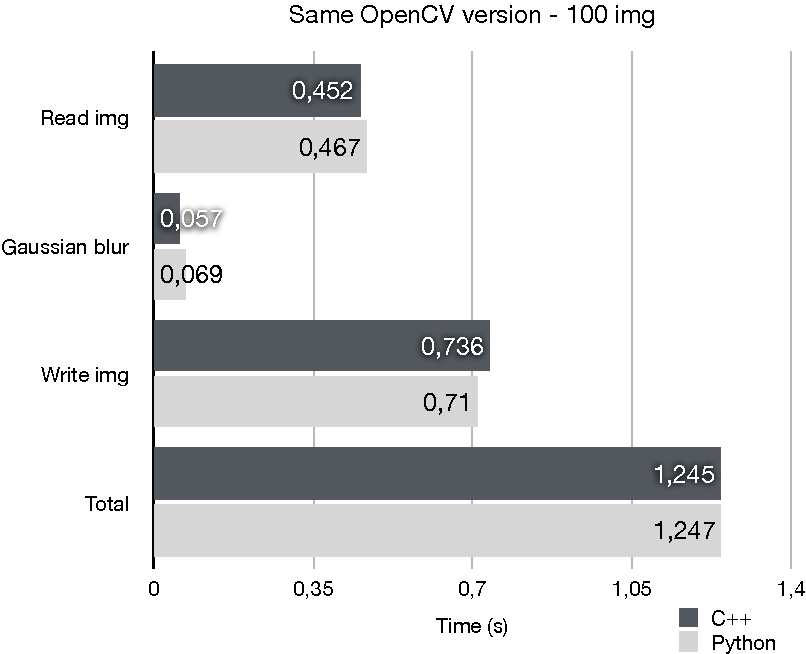
\includegraphics[scale=0.72]{same-opencv.pdf}
	\caption{Average of results using the same OpenCV version}
	\label{figure:same-opencv}
\end{figure}

We can see that the total runtime here is significantly less than when using the previous images. This can probably be attributed to the randomly generated images, which seem to have a lower resolution and are therefore faster to be processed. However, this is not important for this study as only the comparison of C++ and Python is of any consequence and not the overall performance.

\section{The error interval}
An error interval is a property of the instrument and the user and will remain the same for all readings taken, provided the scale is linear \cite{errorinterval}. It can be determined by finding the fraction of the smallest readable division on the instrument. In the table displayed in figure 7.9, benchmarking Python has yielded the error intervals in the last row, which are the same for each reading, using the same instrument.

\begin{figure}[H]
	\centering
	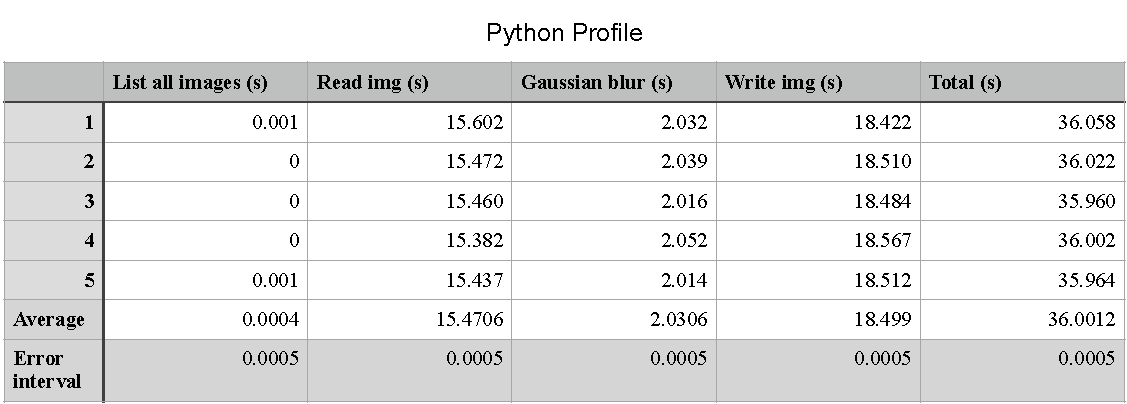
\includegraphics[scale=0.62]{error-interval.pdf}
	\caption{Python profiler average with error interval}
	\label{figure:error-interval}
\end{figure}

From this, it can be determined that if there is a reading of, e.g. 18.500, with an error interval, it is actually between 18.4995 and 18.5005. Whilst this allows for a realistic interpretation of the measurements, it also does not affect any observations since all proportions are still the same.

\section{Energy consumption}
To confirm that runtime was congruous with energy consumption, the Intel Power Gadget was used to approximately measure the energy consumption of each program, both using the standard form of OpenCV with no RAMdisk. C++ had a runtime of 58.233 seconds in the experiment, and Python had a runtime of 38.889 seconds.
Figure 7.10 shows that the proportion of runtime to energy consumption is approximately the same. C++ used more energy than Python for the same program. Python’s runtime is 66.78\% of the C++ runtime, and Python’s energy consumption is 72.00\% of C++’s energy consumption overall and 72.30\% of the energy of the CPU/processor cores. These results indicate that runtime is an approximate indicator of energy consumption.

\begin{figure}[H]
	\centering
	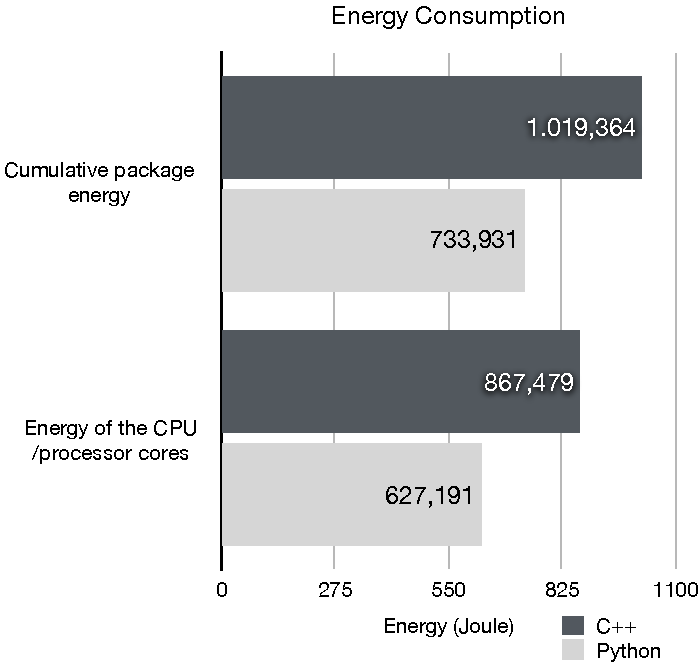
\includegraphics[scale=0.72]{energy.pdf}
	\caption{Energy consumption of the programs in Joule}
	\label{figure:energy-consumption}
\end{figure}
